% !TEX root = main.tex

\chapter{Lenguaje de programaci\'on}
\label{chapter.lang}

Este cap\'itulo presenta una propuesta de un lenguaje de programaci\'on basado en el modelo $\SCCP$ definido en el Cap\'itulo~\ref{chapter.sccp} y cuya sem\'antica operacional est\'a dada por la teor\'ia de reescritura en el Cap\'itulo~\ref{chapter.rew}. La principal raz\'on para crear este lenguaje es permitir a los programadores tener una medio m\'as sencillo para modelar sistemas distribuidos de informaci\'on.  

La Secci\'on~\ref{ebnf.lang} presenta la sintaxis del lenguaje de programaci\'on en la notaci\'on EBNF. La Secci\'on~\ref{sccp.lang} muestra c\'omo el lenguaje esta relacionado con el modelo $\SCCP$ descrito en el Cap\'itulo~\ref{chapter.sccp}. La Secci\'on~\ref{new.lang} presenta una explicaci\'on de los nuevos elementos del lenguaje. Por \'ultimo, la Secci\'on~\ref{example.lang} contiene algunos ejemplos del funcionamiento del lenguaje de programaci\'on.

%% Secci\'on:  %%
\section{EBNF del lenguaje}
\label{ebnf.lang}

EBNF (del ing\'es, \textit{Extended Backus-Naur Form}) es un metalenguaje utilizado para definir formalmente la sintaxis de gram\'aticas libres de contexto, que utiliza expresiones regulares para permitir escribir especificaciones compactas~\cite{ebnfdoc}. 

Una descripci\'on EBNF es una lista no ordenada de reglas EBNF. Cada una de las reglas EBNF esta compuesta de tres partes: el lado izquierdo, el lado derecho y el s\'imbolo `$::=$' separando los dos lados, este s\'imbolo debe ser leido ``se define como''~\cite{ebnfdoc}. El lado izquierdo contiene una palabra escrita en min\'uscula y cursiva delimitada por los caracteres `$\langle$' y `$\rangle$', la cual indica el nombre de la regla EBNF. En el lado derecho se encuentra la definici\'on asociada a este nombre. 

Los nombres asignados en el lado izquierdo de las reglas EBNF pueden ser utilizados como parte de la definici\'on asociada en el lado derecho de las reglas, inclusive dentro de la misma regla, es decir, que puede haber recursi\'on en la descripci\'on del lenguaje.

Las reglas EBNF pueden incluir diez caracteres con significado especial: `$::=$', `$|$', `$+$', `$*$', `$[$', `$]$', `$($', `$)$', `$?$' y `$;$'. Todos los dem\'as caracteres diferentes de los listados anteriormente y de los nombres de las reglas EBNF se definen por si mismos (v.gr., letras, d\'igitos, signos de puntuaci\'on). A continuaci\'on se presenta una explicaci\'on de algunos de los caracteres especiales:

\begin{itemize}
\item Cada regla EBNF debe finalizar con el caracter `$;$'. 
\item `$*$' es un operador unario posfijo, el cual indica que la expresi\'on aparece cero o m\'as veces. 
\item `$+$' es un operador unario posfijo, el cual indica que la expresi\'on aparece una o m\'as veces.
\item `$?$' es un operador unario posfijo, el cual indica que la expresi\'on aparece cero o una vez.
\item M\'ultiples opciones en la definici\'on de un regla EBNF deben estar separadas por el caracter `$|$'.
\item Todas las expresiones delimitadas por comillas simples aparecen de la misma forma en el lenguaje de programaci\'on.
\end{itemize}

\begin{figure}

\begin{flalign*}
\nterm{system} & ::= \nterm{variables}* \nterm{body} \ ; \\
\nterm{variables} & ::= \textterm{var} \nterm{id}+ \ (\textterm{Int} | \textterm{Bool}) \ ; \\
\nterm{body} & ::= \textterm{begin} \nterm{processline}+ \ \textterm{end} \ ; \\
\nterm{processline} & ::= \nterm{process} \textterm{.}  \ ; \\
\nterm{process} & ::= \textterm{tell(} \ \nterm{constraint}  \textterm{)} \ ; \\
	& \bor \textterm{ask} \ (\textterm{<} \ \nterm{location} \textterm{>})? \ \nterm{constraint} \textterm{->}  \nterm{process} \ ; \\
	& \bor \nterm{process} \textterm{||}  \nterm{process} \ ; \\
	& \bor  \textterm{[}  \nterm{process}  \textterm{]\_} \ \nterm{integer} \ ; \\
\nterm{constraint} & ::= \nterm{boolean} \ ; \\
	& \bor \nterm{id} \ ; \\
	& \bor \nterm{expression} \ ; \\
	& \bor \nterm{constraint} \ \textterm{and} \ \nterm{constraint} \ ; \\
\nterm{location} & ::= \nterm{integer} (\textterm{.} \nterm{integer})* \ ; \\
\nterm{expression} & ::= \nterm{id} \nterm{operator} ( \nterm{id} \ | \ \nterm{integer} ) \ ; \\
\nterm{operator} & ::= \textterm{>} \ | \ \textterm{<} \ | \ \textterm{=} \ | \ \textterm{=/=} \ | \ \textterm{>=} \ | \ \textterm{<=} \ ; \\
\nterm{boolean} & ::= \textterm{true} \ | \ \textterm{false} \ ; \\
\nterm{integer} & ::= \textnormal{[0-9]}+ \ ; \\
\nterm{id} & ::= \textnormal{[A-Z] [A-Z0-9]}* \ ;  
\end{flalign*}

\caption{EBNF del lenguaje de programaci\'on.}
\label{fig:ebnf}
\end{figure}

En la Figura~\ref{fig:ebnf} se presenta la descripci\'on EBNF del lenguaje de programaci\'on propuesto. La explicaci\'on de cada una de las reglas EBNF se presenta en las secciones~\ref{sccp.lang} y ~\ref{new.lang}.

%% Secci\'on:  %%
\section{Relaci\'on con $\SCCP$}
\label{sccp.lang}

El lenguaje de programaci\'on que se propone est\'a basado en el modelo $\SCCP$ presentado en el Cap\'itulo~\ref{chapter.sccp}, y es ejecutado en el ambiente de Maude por medio de la especificaci\'on formal presentada en el Cap\'itulo~\ref{chapter.rew}. Por esta raz\'on el lenguaje debe proveer la sintaxis parar los procesos que se han definido hasta el momento. 

Esta secci\'on contiene una explicaci\'on de la relaci\'on entre la definici\'on de $\SCCP$ y algunas de las reglas EBNF de la Figura~\ref{fig:ebnf}. En primer lugar se define el identificador de un agente denominado \cde{location}.

\begin{itemize}
\item \nterm{integer} est\'a definido como cualquier valor entre 0 y 9 repetido una o m\'as veces.
\item \nterm{location} est\'a definido como un \nterm{integer} unido a cero o m\'as repeticiones de un `\cde{.}' y un \nterm{integer}.
\end{itemize}

Los procesos que se describen en la Definici\'on~\ref{def:gensyn} y la Secci\'on~\ref{syntax.rew} son nombrados \nterm{process}, para definirlo se requiere de algunos elementos adicionales, entre los que se encuentran, la definici\'on de un banco de informaci\'on de un agente o la restricci\'on como argumento de un proceso, nombrado \nterm{constraint}. Estos elementos se explican a continuaci\'on:

\begin{itemize}
\item \nterm{boolean} est\'a definido como cualquier valor entre \cde{true} y \cde{false}.
\item \nterm{operator} est\'a definido como cualquier valor entre \textterm{>}, \textterm{<}, \textterm{=}, \textterm{=/=}, \textterm{>=} y \textterm{<=}.
\item \nterm{expression} est\'a definido como un \nterm{id}, seguido de un \nterm{operator} y un \nterm{id} o un \nterm{integer}. 
\item \nterm{constraint} est\'a definido como cualquier opci\'on entre \nterm{boolean}, \nterm{id}, \nterm{expression} y dos \nterm{constraint} unidos por una conjunci\'on l\'ogica (i.e., \textterm{and}).
\end{itemize}

Un proceso, denominado \nterm{process} en el lenguaje de programaci\'on, hace referencia a los 5 procesos del modelo$\SCCP$, incluyendo la extensi\'on de \ask \ descrita de la Secci\'on~\ref{syntax.rew}. La sintaxis es similar a la presentada en la especificaci\'on formal. El proceso \tell \ debe incluir un \nterm{constraint} contenido entre par\'entesis. El proceso \ask \ contiene un \nterm{constraint} y un \nterm{process}, y puede incluir un elemento de tipo \nterm{location} relacionando al identificador de un agente de menor jerarqu\'ia. El proceso de ejecuci\'on en paralelo contiene los procesos a ser ejecutados en paralelo. Finalmente, el proceso de especificaci\'on del espacio de ejecuci\'on requiere del proceso a ejecutar \nterm{process} y un numero \nterm{integer} referente al identificador del agente de menor jerarqu\'ia donde se va a ejecutar el proceso.

%% Secci\'on:  %%
\section{Nuevas caracter\'isticas}
\label{new.lang}   

Debido a que el objetivo del lenguaje propuesto es brindar a los programadores un medio m\'as sencillo para modelar sistemas distribuidos de informaci\'on por medio del modelo $\SCCP$, se incluyen algunas caracter\'isticas que faciliten el uso del lenguaje y la especificaci\'on de un sistema, como la declaraci\'on de variables.

Un programa \nterm{system} tiene dos partes: el encabezado \nterm{variables} y el cuerpo \nterm{body}. El encabezado contiene la declaraci\'on de las variables a las cuales se les asigna un nombre \nterm{id} y un tipo (v.gr., \textterm{Int} o \textterm{Bool}), por ejemplo la sentencia \cde{var X T Int} indica que \cde{X} y \cde{T} son variables de tipo entero. Un programa puede incluir cero o m\'as declaraciones, y un \nterm{id} no puede corresponder a dos variables de diferentes tipos. Toda variable utilizada dentro del cuerpo del programa debe estar declarada en el encabezado, de lo contrario se producir\'a un error en la compilaci\'on del programa respectivo.  

El cuerpo del programa debe comenzar con la palabra \textterm{begin} y finalizar con \textterm{end}; si alguna de estas palabras no se incluye se producir\'a un error en la compilaci\'on. Cada l\'inea del cuerpo del programa debe corresponder a uno de los procesos explicados en la Secci\'on~\ref{sccp.lang} finalizada con el caracter \textterm{.}. El interprete omite todas las lineas que se encuentren despu\'es de la palabra \textterm{end}.

%% Secci\'on:  %%
\section{Ejemplo}
\label{example.lang}

Para mayor claridad en el uso del lenguaje de programaci\'on en la Secci\'on~\ref{example.lang} se presentan algunos ejemplos. Considere el ejemplo que se trabaj\'o en las secciones~\ref{example.sccp} y~\ref{example.rew}. El programa requerido para obtener el estado inicial del sistema $d$ se presenta a continuaci\'on: 

\begin{sccp}
var V W X Y Z Int
begin
tell(V > 10) .
[tell(W = 3)]_1 || [[tell(X = 17)]_3]_1 .
[tell(Y > 4)]_2 || [[tell(Z = 20)]_1]_2 .
end
\end{sccp}

Todas los procesos pueden ser escritos en una sola l\'inea utilizando procesos en paralelo; para facilidad en la lectura en el ejemplo anterior se presentan m\'ultiples l\'ineas de forma que se genera el \'arbol de la Figura~\ref{fig:sccptree} de izquierda a derecha. Ahora se definene los procesos $R$, $P$ y $Q$ respectivamente como:

\begin{sccp}
[tell(V = 42)]_3 || tell(T = 8)
ask Y > 0 -> tell(Z > 10) 
ask T > 7 -> [tell(S =/= 2)]_2 
\end{sccp}

Con los procesos $R$, $P$ y $Q$ se construye $S$ y se agrega al estado inicial para alcanzar el estado final del sistema presentado en la Figura~\ref{fig:sccptree2}. El programa correspondiente se muestra a continuaci\'on:

\begin{sccp}
var V W X Y Z Int
var S T Int
begin
tell(V > 10) .
[tell(W = 3)]_1 || [[tell(X = 17)]_3]_1 .
[tell(Y > 4)]_2 || [[tell(Z = 20)]_1]_2 .
[[tell(V = 42)]_3 || tell(T = 8)]_1 || 
[ask Y > 0 -> tell(Z > 10) ]_2 || 
[ask T > 7 -> [tell(S =/= 2)]_2 ]_1 .
end
\end{sccp}

Tal como se indic\'o en la Secci\'on~\ref{new.lang} un proceso debe terminar con el caracter \textterm{.}, por lo tanto cuando el proceso es extenso como $S$ puede ser separado en m\'ultiples l\'ineas para facilitar su manejo. En este cap\'itulo se presenta el programa que lleva al estado final del sistema; su ejecuci\'on y verificaci\'on se realiza en el Cap\'itulo~\ref{chapter.envir}.

Considere otro sistema descrito por el siguiente programa: 

\begin{sccp}
var B0 B1 Bool
var X C Int
var Y B Int
begin
tell(true) .
ask true -> tell(X >= 5) .
[[tell(B0)]_1 || ask < 1 > B0 -> tell(Y < X)]_1 .
tell(true) || ask X > 1 -> tell(B1) .
[tell(X >= 5)]_2 .
ask B1 -> tell(C >= 5) .
end
\end{sccp}

A partir del programa descrito anteriormente, el estado final esperado del sistema es representado en la Figura~\ref{fig:langexample}. Debido a que la informaci\'on que tiene o transmite un agente simboliza relaciones o restricciones sobre las variables del sistema, el banco de infomaci\'on de un agente puede ser representado por elementos de tipo \cde{Bool}, tal como las variables \cde{B0} y \cde{B1}. 

\begin{figure}[htbp] %  figure placement: here, top, bottom, or page
   \centering
   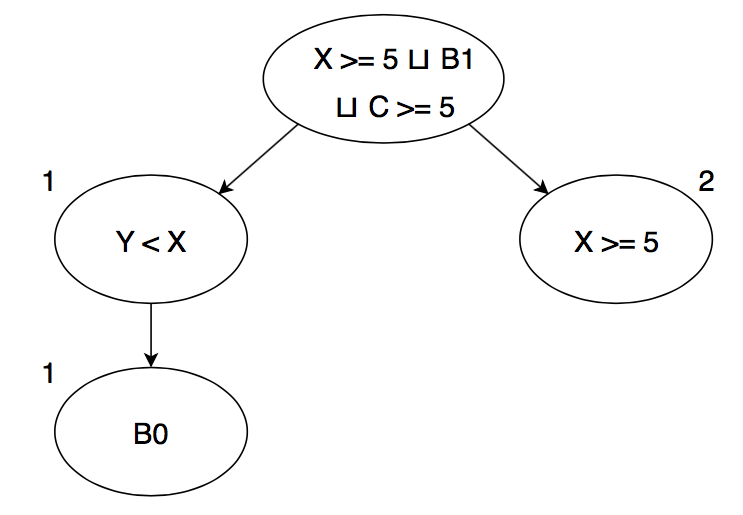
\includegraphics[width=3.5in]{langexample.png} 
   \caption{Estado inicial ejemplo$\SCCP$}
   \label{fig:langexample}
\end{figure}

La ejecuci\'on y verificaci\'on del programa se realiza en el Cap\'itulo~\ref{chapter.envir}.

